%%
% Please see https://bitbucket.org/rivanvx/beamer/wiki/Home for obtaining beamer.
%%
%\documentclass[11pt,aspectratio=169]{beamer}
%\documentclass[11pt,aspectratio=169,xcolor={dvipsnames}]{beamer}

\documentclass[11pt,aspectratio=169,xcolor={dvipsnames},hyperref={pdftex,pdfpagemode=UseNone,hidelinks,pdfdisplaydoctitle=true},usepdftitle=false]{beamer}
\usepackage{presentation}


\title{Lecture 20: Lumpy Investment in GE}
\author{Juan Herre\~{n}o\\UCSD}
\date{2026}

% Enter presentation title to populate PDF metadata:
\newcommand{\Cov}{\text{Cov}_\lambda}
\newcommand{\El}{\mathbb{E}_\lambda}
\newcommand{\mm}{\text{{\fontfamily{qzc}\selectfont m}}}
\usepackage{cancel}
\usepackage{booktabs}
\usepackage{dsfont}
\usepackage{tikz}

\begin{document}

\maketitle

\begin{frame}{Outline of this lecture}
\begin{itemize}
\item In this lecture, we plug our heterogeneous-firm blocks into a GE model
\item With the purpose of:
\begin{itemize}
\item In what way does general equilibrium adjustment change the implications of partial equilibrium models?
\item Are microeconomic frictions relevant for understanding macro effects of, say, tax policy?
\end{itemize}
\end{itemize}
\end{frame}



\begin{frame}{Generic Setting}
Firms have a DRS production function
$$y = e^z e^{a} k^{\alpha} n^{\gamma}$$
$a$ captures idiosyncratic productivity (iid across firms)
$$a_{it} = \rho_a a_{i,t-1} + \epsilon_{it} \sigma_a.$$
$z$ captures aggregate productivity
$$z_{t} = \rho_z z_{t-1} + \xi_{t} \sigma_z.$$
Firms discount period $\tau$ future profits with the household stochastic discount factor $\Lambda_{t,t+\tau}$
\end{frame}


\begin{frame}{Generic Setting}
$$V(k,a,\chi,\mathcal{S}) = \max_n \left[e^z e^{a} k^{\alpha} n^{\gamma} - w(\mathcal{S}) n\right] + \max \left[V^n(k,a,\chi, \mathcal{S}),V^a(k,a,\chi,\mathcal{S}) - \chi w(\mathcal{S}) \right]$$ \vspace{-0.5cm}
The value function conditional on non-adjustment is given by:

$$V^n(k,a,\chi,\mathcal{S}) = \mathbb{E}(\Lambda(\mathcal{S},\mathcal{S'}) V(k',a',\chi',\mathcal{S'})|a,\mathcal{S}),$$ subject to $$k' = k(1-\delta)$$ \vspace{-0.5cm}

The value function conditional on adjustment is given by:

$$V^a(k,a,\chi,\mathcal{S}) = \max_i \left\{- i -\phi \left(\frac{i}{k}\right)^2 k +  \mathbb{E}\left[\Lambda(\mathcal{S},\mathcal{S'}) V(k',a',\chi',\mathcal{S'}) \mid a,\mathcal{S}\right]\right\},$$ subject to $$k' = k(1-\delta) + i$$. \vspace{-0.5cm}
\end{frame}

\begin{frame}{Generic setting}
In the background there is a representative household that supplies labor, and consumes.
\begin{itemize}
\item There is a labor supply function in the background
\item The Stochastic Discount Factor will capture household preferences for consumption smoothing
\end{itemize}
\end{frame}

\begin{frame}{The state space}
\begin{itemize}
\item The state space is given by $(k,a,\mathcal{S})$
\item In particular, $(\mathcal{S})$ captures the aggregate state space. What is in it?
\item Easy part: It includes $z$. $\mathcal{S} = \mathcal{H}(\Gamma,z)$. 
\item What is in $\Gamma$ ?
\end{itemize}
\end{frame}

\begin{frame}{What is the state?}
\begin{itemize}
\item Generic answer: All variables that affect firm's value must be determined by the state.
\item $\mathcal{S} = \mathcal{H}(\Gamma,z)$.
\item $\Gamma$ is the distribution of firms over their individual state-space $(a,k,\chi)$
\item Why is $\Gamma$ a relevant object for these firms?
\item To make intertemporal choices, firms must forecast the future. Two aspects
\begin{itemize}
\item They need to forecast tomorrow's wage rate. $w(\mathcal{S'})$
\item They need to forecast tomorrow's SDF $\Lambda(S',S'')$.
\item With $\Gamma$ it is possible to forecast future labor demand and supply, and back out the market-clearing wage
\item It is not possible to forecast $w$ without knowing $\Gamma$ in general.
\end{itemize}
\end{itemize}
\end{frame}

\begin{frame}{The Curse of Dimensionality}
\begin{itemize}
\item $\mathcal{S}$ creates an important computational challenge
\item $\Gamma$ is an infinite-dimensional object $\Gamma(a,k,\chi)$. Joint distribution on $\mathbb{R} \times \mathbb{R^+}\times \mathbb{R}^+$
\item We could discretize the state-space. Imagine $k_n = 100$, $a_n = 2$, and $\chi$ iid. $\Gamma$ adds 200 state variables
\item The mass of firms in each of the $(k,a)$ bins.
\item Still impossible to implement in modern computers
\item Approximations as outlined in the Menu Cost lecture
\end{itemize}
\end{frame}


\begin{frame}{Thomas 2002}
\begin{itemize}
\item Research Question: Does lumpy adjustment of capital affect aggregate investment dynamics in an otherwise standard general equilibrium business cycle model?
\item Remember: RBC model close to linear
\item Lumpy investment model had a state-dependent response of investment
\item Conclusion
\begin{itemize}
\item No!
\item ``Lumpy investment appears largely irrelevant for equilibrium business cycle analysis''
\item Quantitative dynamics of macro aggregates are virtually indistinguishable from a frictionless RBC model
\end{itemize}
\end{itemize}
\end{frame}




\begin{frame}{Thomas 2002}
\begin{itemize}
\item Productivity $A_t = X_t z_t$
\item Trend growth in productivity $X_t = X_{t-1}\Psi_A$
\item Stochastic aggregate productivity $z_t = \rho z_{t-1} + \xi_t$
\item Standard household behavior $U(C_t,L_t)$.
\end{itemize}
\end{frame}



\begin{frame}{Thomas 2002}
\begin{itemize}
\item Thomas (2002) simplifies the generic framework we detailed in a number of ways
\item Worth detailing a couple of them
\begin{itemize}
\item Firms face non-convex costs but do not face convex costs
\item Firms face aggregate productivity shocks but do not face idiosyncratic productivity shocks
\end{itemize}
\end{itemize}
\end{frame}

\begin{frame}{Thomas 2002}
Cross-sectional distribution of plants.
\begin{itemize}
\item Remember, in principle need to track the mass of firms in the state-space
\item But symmetry (no convex costs, no idiosyncratic shocks) implies that all firms that adjust at time $t$ choose the same $k_{0,t+1}$
\item Can keep track of the capital across \textit{vintages} rather than firms
$$k_{0,t+1} = (1-\delta)k_{j,t} + i_{j,t}$$
$$k_{j+1,t+1} = (1-\delta) k_{j,t}$$
\end{itemize}
\end{frame}


\begin{frame}{Thomas 2002}
\begin{itemize}
\item As in Caballero and Engel (1999), adjustment hazards are increasing in capital imbalances
\item Assumption $\chi \sim U(0,B)$
\item There exists a cutoff for the fixed cost $\bar{\chi}_j$ such that firms with vintage $j$ adjust iff $\chi < \bar{\chi}_j$
\item The probability of adjustment for firms with vintage $j$ is noted by $\alpha_{j,t}$	
%$$w_t G^{-1}(\alpha_{j,t} + i_{j,t}) = v_{0,t} - v_{j+1,t}$$
\item There exists $J$ sufficiently large such that $\alpha_{J,t} = 1$
\item Clever: Transformed a problem with infinitely many state variables, into a problem with $J$ states.
\end{itemize}
\end{frame}




\begin{frame}{Thomas 2002}
\begin{itemize}
\item The problem of individual firms is not smooth
\item Planner's problem is smooth: summarized by $\alpha$.
\item Possible to linearize
\item Finite number of vintages $\rightarrow$ finite number of states.
\end{itemize}
\end{frame}

\begin{frame}{Thomas 2002}
\begin{figure}
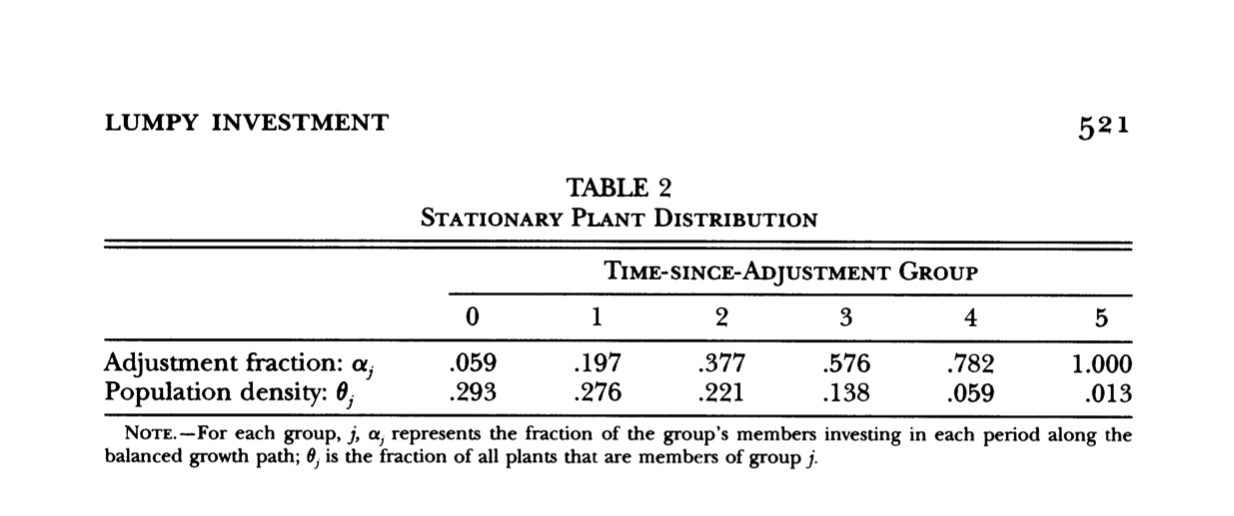
\includegraphics[scale=0.6]{FiguresTables/t_1}
\end{figure}
\end{frame}


\begin{frame}{Thomas 2002}
\begin{figure}
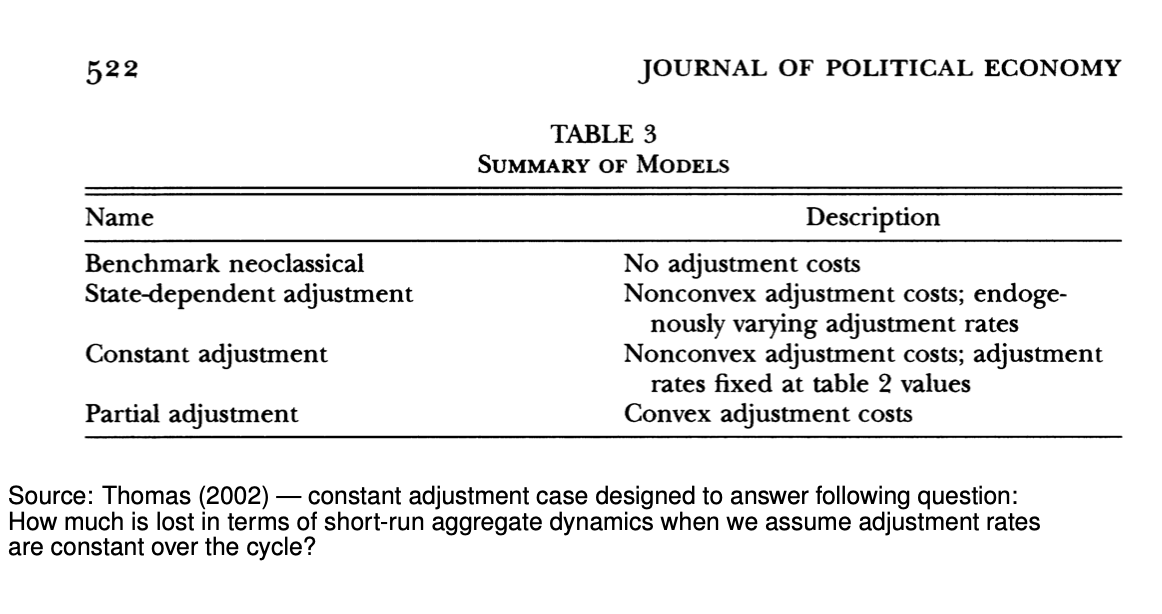
\includegraphics[scale=0.6]{FiguresTables/t_2}
\end{figure}
\end{frame}


\begin{frame}{Thomas 2002}
\begin{figure}
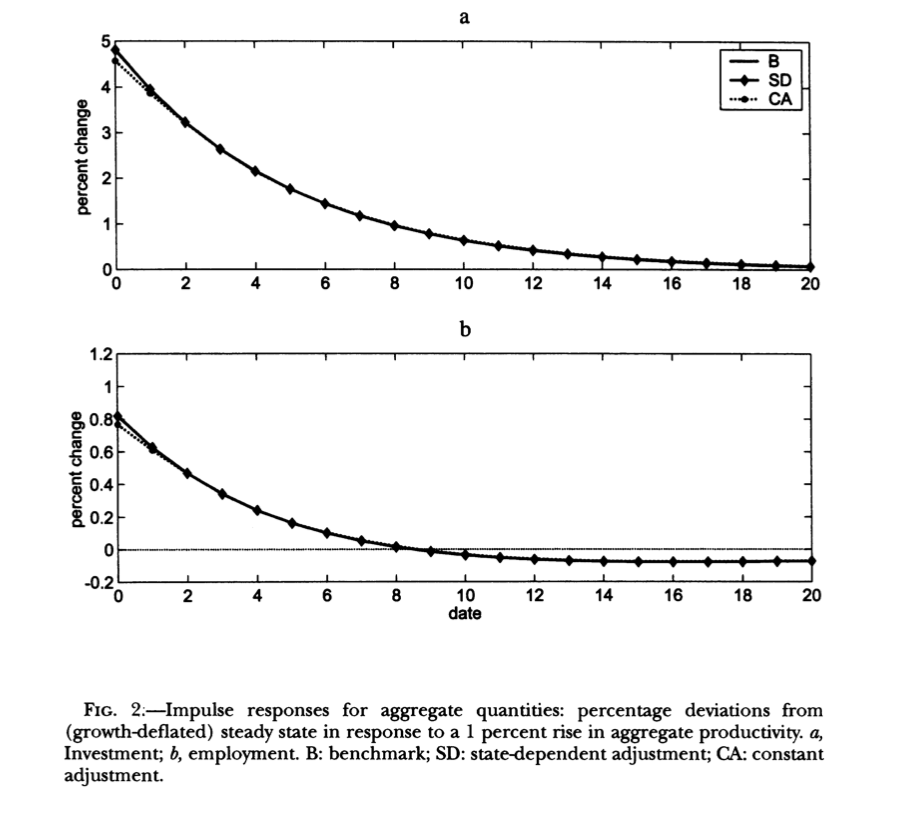
\includegraphics[scale=0.5]{FiguresTables/t_3}
\end{figure}
\end{frame}

\begin{frame}{Khan and Thomas 2008}
\begin{itemize}
\item Some debate on whether the results were the outcome of the very specific modeling choices
\item Khan and Thomas (2008) find pretty much the same results in a model that looks closer to what we wrote in this lecture note

$$ U(c,L) = \log c + \varphi L$$
\end{itemize}
\end{frame}

\begin{frame}{Khan and Thomas 2008}
\begin{figure}
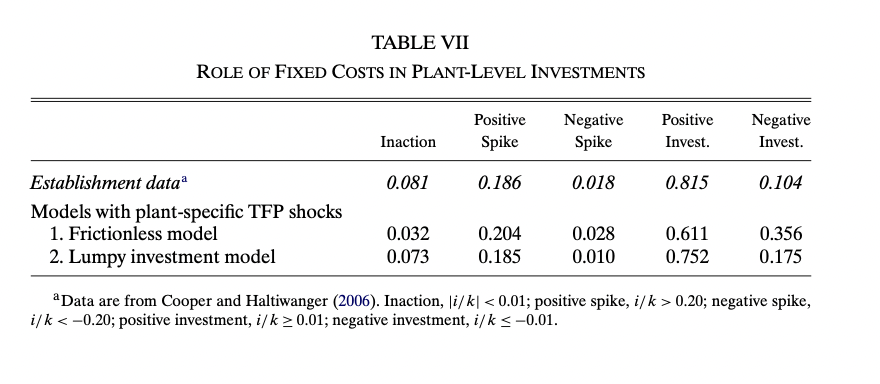
\includegraphics[scale=0.45]{FiguresTables/kt_1}
\end{figure}
\end{frame}


\begin{frame}{Khan and Thomas 2008}
\begin{figure}
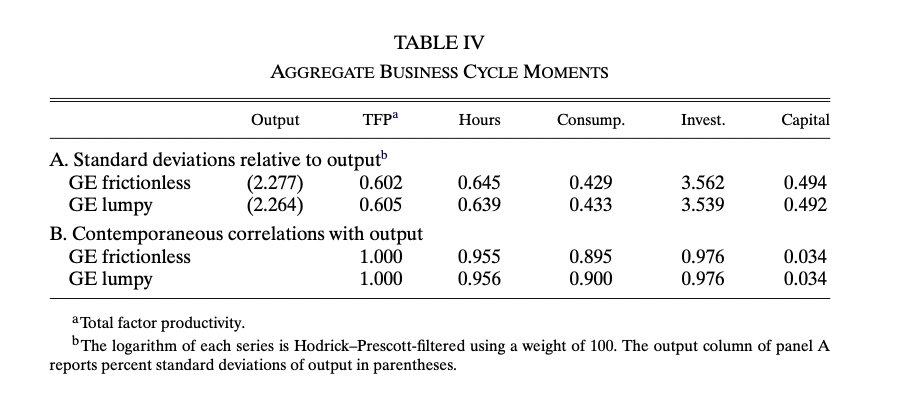
\includegraphics[scale=0.45]{FiguresTables/kt_2}
\end{figure}
\end{frame}


\begin{frame}{Rough intuition}
\begin{itemize}
\item $\alpha$ returns to scale (CRS: $\alpha = 1$).
$$\frac{\partial i_{jt}/i_{jt}}{\partial r_t} = - \frac{1}{1-\alpha}\frac{1}{\delta}\frac{1+r_t}{r_t + \delta}$$
\item When $\alpha \rightarrow 1$, the investment of unconstrained firms is infinitely elastic
\item Small changes in aggregate prices induce infinite responses
\end{itemize}
\end{frame}


\begin{frame}{Winberry 2021}
$$\frac{\partial i_{jt}/i_{jt}}{\partial r_t} = - \frac{1}{1-\alpha}\frac{1}{\delta}\frac{1+r_t}{r_t + \delta}$$
\begin{itemize}
\item Under a reasonable calibration:
\item $\alpha = 0.7$, $\delta = 0.025$, $r_t = 0.01$: $\frac{\partial i_{jt}/i_{jt}}{\partial r_t} = -3,847$
\item $r_t$ is an equilibrium outcome, so much depends on how $r_t$ behaves.
\item The standard model has very strong strategic substitutability
\item That others do not adjust induces higher incentives to adjust
\item Mediated by the response of the real interest rate to aggregate shocks
\end{itemize}
\end{frame}

\begin{frame}{Winberry 2021}
\begin{figure}
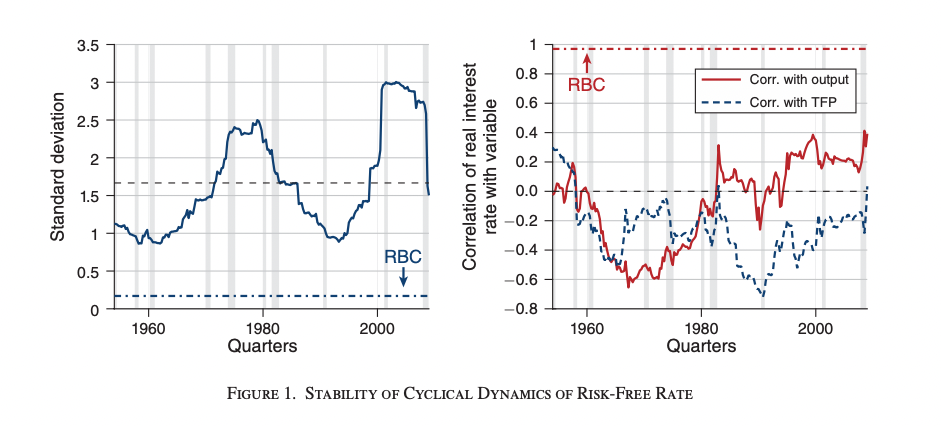
\includegraphics[scale=0.45]{FiguresTables/w_1}
\end{figure}
\end{frame}


\begin{frame}{Winberry 2021}
\begin{figure}
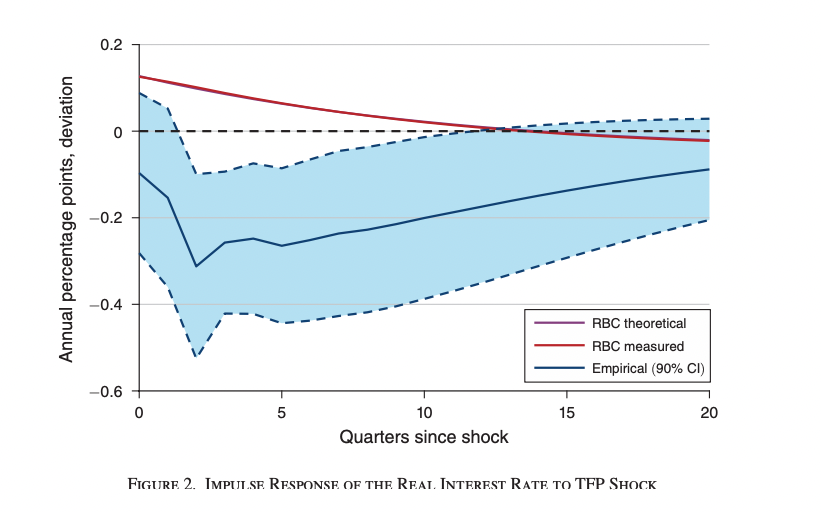
\includegraphics[scale=0.45]{FiguresTables/w_2}
\end{figure}
\end{frame}



\begin{frame}{Habits in Consumption}
\begin{itemize}
\item Fix the dynamics of $r$ by changing optimal consumption decisions
$$\mathbb{E}_t \sum_{t=0}^{\infty} \beta^t \left[\log C_t - \chi \frac{N^{1+\xi}_t}{1+\xi} - X_t \right]$$
$$X_t = \lambda \hat{C}_t$$
$$\hat{C}_t = C_t - \chi \frac{N^{1+\xi}_t}{1+\xi}$$
\end{itemize}
\end{frame}


\begin{frame}{Winberry 2021}
\begin{figure}
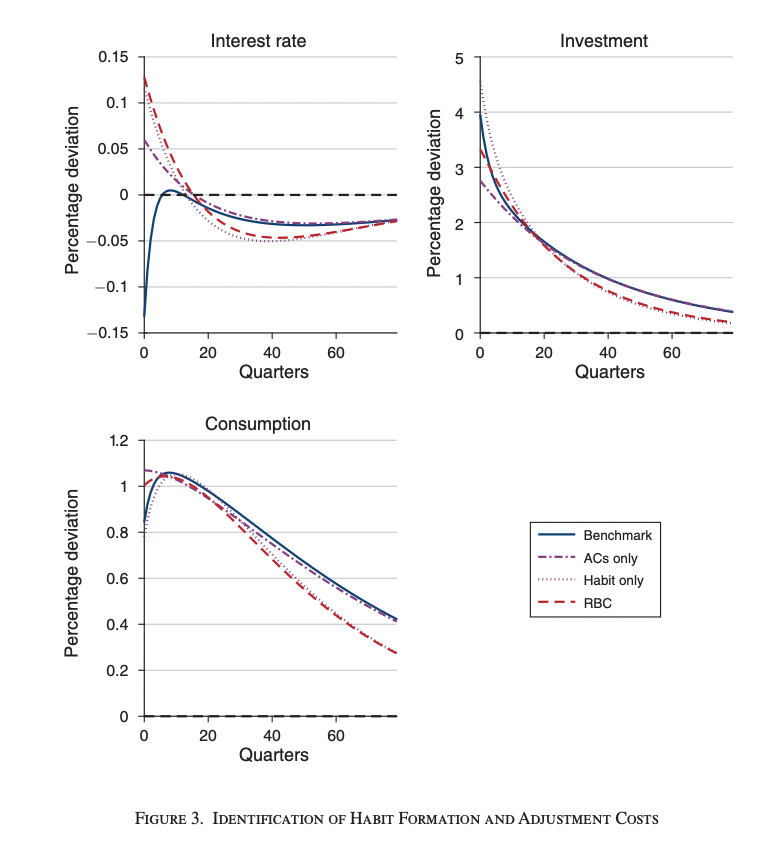
\includegraphics[scale=0.25]{FiguresTables/w_4}
\end{figure}
\end{frame}


\begin{frame}{Winberry 2021}
\begin{figure}
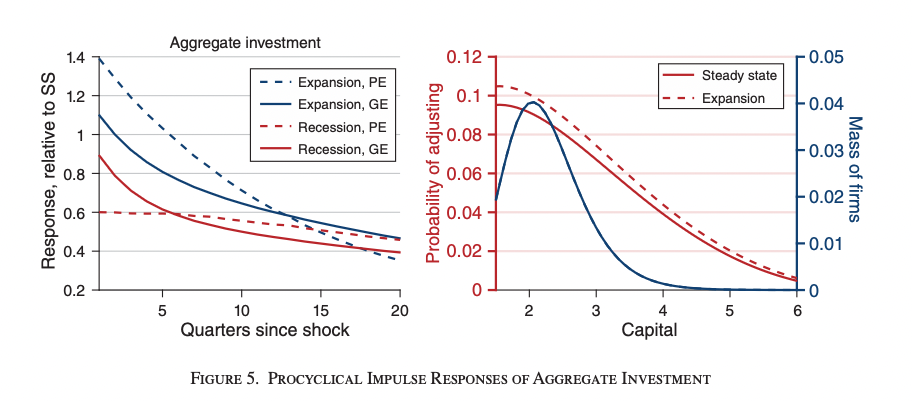
\includegraphics[scale=0.45]{FiguresTables/w_3}
\end{figure}
\end{frame}

\begin{frame}{Koby and Wolf 2022}
\begin{itemize}
\item The PE semi-elasticity of investment to interest rates in Khan and Thomas (2008) = 500\%
\item In Winberry (2021) is roughly 7\%
\item Meaning: In Khan and Thomas, interest rates need to increase 71 times less to accommodate the same change in investment demand
\item How to choose?
\item Zwick and Mahon cross-sectional responses imply a semi-elasticity close to Winberry's
\item 100 times smaller than that of Khan and Thomas (2008)
\end{itemize}
\end{frame}

\begin{frame}{Koby and Wolf 2022}
\begin{itemize}
\item Why is Zwick and Mahon (2017) evidence relevant?
\item Because it answers precisely the question of:
\begin{center}
\textit{After differencing-out general equilibrium responses, how much more investment occurs at a firm that faces a smaller cost of capital relative to a firm that has a higher cost of capital?}
\end{center}
\item Note that Zwick and Mahon (2017) do not answer the macro question
\item But their evidence let us to distinguish across macro models
\end{itemize}
\end{frame}


\begin{frame}{Messages}
\begin{itemize}
\item GE effects can undo lessons in PE
\item But there is not a single way to aggregate
\item Cross-sectional evidence can be useful to distinghish across models
\end{itemize}
\end{frame}

\begin{frame}{Policy Messages}
\begin{itemize}
\item Tax policy is less effective in recessions
\item More firms are likely to make an extensive margin investment in expansions than in recessions
\end{itemize}
\end{frame}




\end{document}



